\imprimircapa

\imprimirfolhaderosto*

\begin{fichacatalografica}
	\vspace*{\fill}
	\begin{center}
		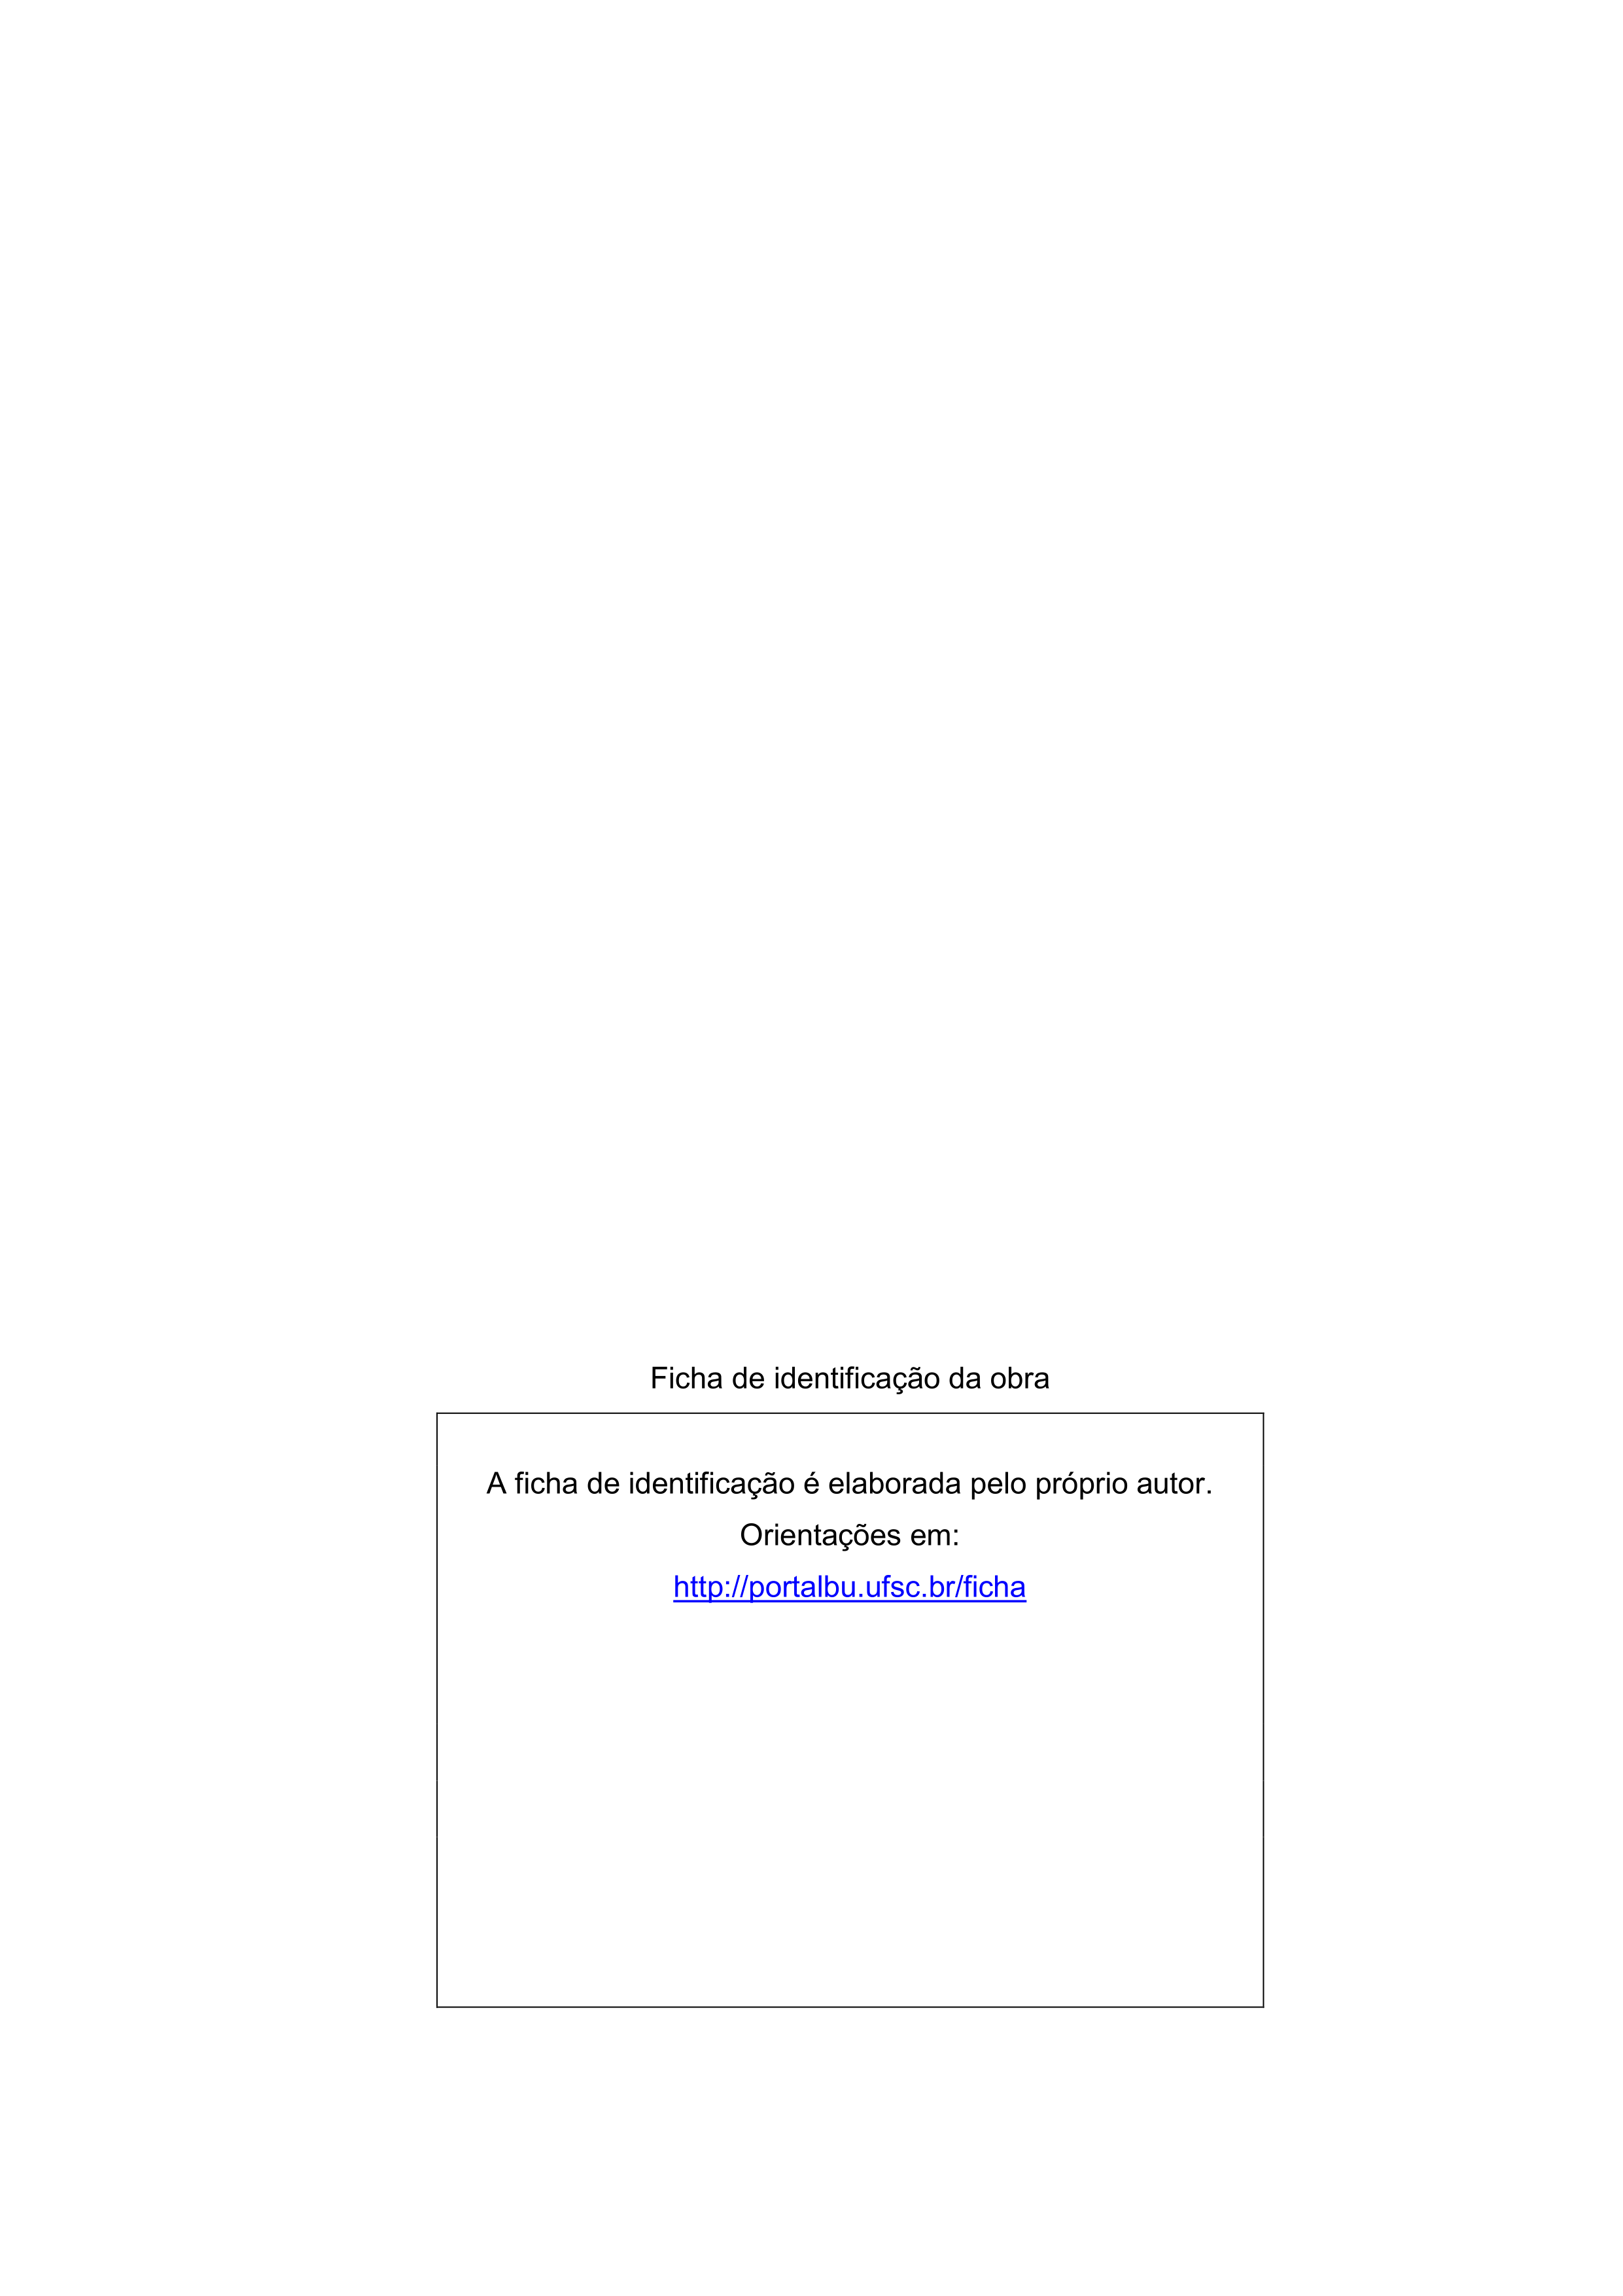
\includegraphics[width=\textwidth,height=0.85\textheight,keepaspectratio]{beforetext/Ficha_Catalografica.png}
	\end{center}
	\vspace*{\fill}
\end{fichacatalografica}

\begin{folhadeaprovacao}
	\OnehalfSpacing
	\centering
	\imprimirautor\\
	\vspace*{10pt}
	\textbf{\imprimirtitulo}
	\ifnotempty{\imprimirsubtitulo}{:~\imprimirsubtitulo}\\
	\vspace*{\baselineskip}
	O presente trabalho em nível de \imprimirnivel~foi avaliado e aprovado, em \imprimirdata, pela banca examinadora composta pelos seguintes membros:\\
	\vspace*{\baselineskip}
	Prof.(a) xxxx, Dr(a).\\
	Instituição xxxx\\
	\vspace*{\baselineskip}
	Prof.(a) xxxx, Dr(a).\\
	Instituição xxxx\\
	\vspace*{\baselineskip}
	Prof.(a) xxxx, Dr(a).\\
	Instituição xxxx\\
	\vspace*{2\baselineskip}
	\begin{minipage}{\textwidth}
		Certificamos que esta é a \textbf{versão original e final} do trabalho de conclusão que foi julgado adequado para obtenção do título de \imprimirformacao.\\
	\end{minipage}
	\vspace*{\fill}
	\assinatura{\OnehalfSpacing Coordenação do Programa de Pós-Graduação}
	\vspace*{\fill}
	\assinatura{\OnehalfSpacing\imprimirorientador \\ \imprimirorientadorRotulo}
	\vspace*{\fill}
	\imprimirlocal, \imprimirano.
\end{folhadeaprovacao}

% TODO: Dedicar
\begin{dedicatoria}
	\vspace*{\fill}
	\noindent
	\begin{adjustwidth*}{}{5.5cm}
		\raggedleft
		...
	\end{adjustwidth*}
\end{dedicatoria}

% TODO: Agradecer
\begin{agradecimentos}
    ...
\end{agradecimentos}

% TODO: Epigrafar
\begin{epigrafe}
	\vspace*{\fill}
	\begin{flushright}
		\textit{...}
	\end{flushright}
\end{epigrafe}

% TODO: Resumir
\setlength{\absparsep}{18pt}
\begin{resumo}
	\SingleSpacing
    ...
	
	\textbf{Palavras-chave}: ...
\end{resumo}

% TODO: Summarize
\begin{resumo}[Abstract]
	\SingleSpacing
	\begin{otherlanguage*}{english}
        ...

		\textbf{Keywords}: ...
	\end{otherlanguage*}
\end{resumo}

{
	\hypersetup{hidelinks}
	\pdfbookmark[0]{\listfigurename}{lof}
	\listoffigures*
	\cleardoublepage
	
	\pdfbookmark[0]{\listofquadrosname}{loq}
	\listofquadros*
	\cleardoublepage
	
	\pdfbookmark[0]{\listtablename}{lot}
	\listoftables*
	\cleardoublepage
	
	\imprimirlistadesiglas
	
	\imprimirlistadesimbolos
	
	\pdfbookmark[0]{\contentsname}{toc}
	\tableofcontents*
	\cleardoublepage
}
